\documentclass{article}

%%%%%%%%%%%%%%%%%%%%%%%%%%%%%%%%%
% PACKAGE IMPORTS
%%%%%%%%%%%%%%%%%%%%%%%%%%%%%%%%%
\usepackage[framemethod=TikZ]{mdframed}
\usepackage{amsthm}
\usepackage{tikzsymbols}
\usepackage[tmargin=2.5cm,rmargin=2cm,lmargin=2.5cm,margin=0.85in,bmargin=2.5cm,footskip=.2in]{geometry}
\linespread{1.3}
\usepackage{amsmath,amsfonts,amsthm,amssymb,mathtools}
\usepackage[varbb]{newpxmath}
\usepackage{xfrac}
\usepackage[makeroom]{cancel}
\usepackage{bookmark}
\usepackage{enumitem}
\usepackage{hyperref,theoremref}
\hypersetup{
	pdftitle={Assignment},
	colorlinks=true, linkcolor=doc!90,
	bookmarksnumbered=true,
	bookmarksopen=true
}
\usepackage[most,many,breakable]{tcolorbox}
\usepackage{xcolor}
\usepackage{varwidth}
\usepackage{etoolbox}
\usepackage{nameref}
\usepackage{multicol,array}
\usepackage{tikz-cd}
\usepackage[ruled,vlined,linesnumbered]{algorithm2e}
\usepackage{comment} % enables the use of multi-line comments (\ifx \fi) 
\usepackage{xifthen}
\usepackage{pdfpages}
\usepackage{transparent}
\usepackage[bottom]{footmisc}
\usepackage[utf8]{inputenc} % allow utf-8 input
\usepackage{braket}
\usepackage{titling} % For customizing title
\usepackage{abstract} % For abstract formatting
\usepackage{wrapfig}			  %Kontekstom osjetljivo navođenje
\usepackage{csquotes}			  %Kontekstom osjetljivo navođenje
\usepackage{graphicx}       %Slike i slično
\usepackage{url}            % simple URL typesetting
\usepackage{booktabs}       % professional-quality tables
\usepackage{nicefrac}       % compact symbols for 1/2, etc.
\usepackage{float}
\usepackage{caption}
\usepackage{subcaption}
\usepackage{listings}
\usepackage[english]{babel}
\usepackage{titlesec}				%Za naslovnu stranicu
\usepackage[T1]{fontenc}
\usepackage{import}
\usepackage{svg}



\counterwithin{figure}{section}
\urlstyle{same}
\numberwithin{equation}{section}
\hyphenation{pergamon} % riječ u argumentu (pergamon) se ne rastavlja s crticom; ne smije imat specijalna slova. č. ž... - rastavljam ju naredbom \- (npr. išče\-zava)
\setlength\parindent{0pt} % u novom paragrafu: indent=0
\setlength{\parskip}{10pt} % postavlja željeni vertikalni razmak između paragrafa
\setlength{\skip\footins}{2cm} % razmak između glavnog teksta i fusnota
\renewcommand{\thefootnote}{$\ddagger$} % želim dagger za oznaku fusnota
\newcommand{\HRule}{\rule{\linewidth}{0.4mm}} % nova naredba za horizontalne linije na naslovnoj stranici
\newlength{\mylen}
\setcounter{secnumdepth}{4}
\titleformat{\paragraph}
{\normalfont\normalsize\bfseries}{\theparagraph}{1em}{}


%%%%%%%%%%%%%%%%%%%%%%%%%%%%%%%%%%%%%%%%%%%
% TABLE OF CONTENTS
%%%%%%%%%%%%%%%%%%%%%%%%%%%%%%%%%%%%%%%%%%%

\usepackage{tikz}
\definecolor{doc}{RGB}{0,60,110}
\usepackage{titletoc}
\contentsmargin{0cm}
\titlecontents{chapter}[3.7pc]
{\addvspace{30pt}
	\begin{tikzpicture}[remember picture, overlay]
		\draw[fill=doc!60,draw=doc!60] (-7,-.1) rectangle (-0.9,.5);
		\pgftext[left,x=-3.5cm,y=0.2cm]{\color{white}\Large\sc\bfseries Chapter\ \thecontentslabel};
	\end{tikzpicture}\color{doc!60}\large\sc\bfseries}
{}
{}
{\;\titlerule\;\large\sc\bfseries Page \thecontentspage
	\begin{tikzpicture}[remember picture, overlay]
		\draw[fill=doc!60,draw=doc!60] (2pt,0) rectangle (4,0.1pt);
	\end{tikzpicture}}
\titlecontents{section}[1.7pc]
{\addvspace{8pt}}
{\contentslabel[\thecontentslabel]{1pc}}
{}
{\ \hrulefill\ \small\thecontentspage}
[\vspace{-0.4cm}]
\titlecontents*{subsection}[3.7pc]
{\addvspace{-0pt}\small}
{}
{}
{\dotfill \small\thecontentspage\\}
[][\vspace{-1cm}]

\makeatletter
\renewcommand{\tableofcontents}{
	\chapter{
	  \vspace{-20\p@}
	  \begin{tikzpicture}[remember picture, overlay]
		  \pgftext[right,x=15cm,y=0.2cm]{\color{doc!60}\Huge\sc\bfseries \contentsname};
		  \draw[fill=doc!60,draw=doc!60] (13,-.75) rectangle (20,1);
		  \clip (13,-.75) rectangle (20,1);
		  \pgftext[right,x=15cm,y=0.2cm]{\color{white}\Huge\sc\bfseries \contentsname};
	  \end{tikzpicture}}
	\@starttoc{toc}}
\makeatother


%%%%%%%%%%%%
%% KUTIJE %%
%%%%%%%%%%%%
%%%%%%%%%%%%%%%%%%%%%%%%%%%%%%
%Theorem
\newcounter{teorem}[section] \setcounter{teorem}{0}
\renewcommand{\theteorem}{\arabic{section}.\arabic{teorem}}
\newenvironment{teorem}[2][]{%
	\refstepcounter{teorem}%
	\ifstrempty{#1}%
	{\mdfsetup{%
			frametitle={%
					\tikz[baseline=(current bounding box.east),outer sep=0pt]
					\node[anchor=east,rectangle,fill=blue!20]
					{\strut Teorem~\thetheo};}}
	}%
	{\mdfsetup{%
			frametitle={%
					\tikz[baseline=(current bounding box.east),outer sep=0pt]
					\node[anchor=east,rectangle,fill=blue!20]
					{\strut Teorem~\thetheo:~#1};}}%
	}%
	\mdfsetup{innertopmargin=10pt,linecolor=blue!20,%
		linewidth=2pt,topline=true,%
		frametitleaboveskip=\dimexpr-\ht\strutbox\relax
	}
	\begin{mdframed}[]\relax%
		\label{#2}}{\end{mdframed}}
%%%%%%%%%%%%%%%%%%%%%%%%%%%%%%
%Proof
\newcounter{dokaz}[section]\setcounter{dokaz}{0}
\renewcommand{\thedokaz}{\arabic{section}.\arabic{dokaz}}
\newenvironment{dokaz}[2][]{%
	\refstepcounter{dokaz}%
	\ifstrempty{#1}%
	{\mdfsetup{%
			frametitle={%
					\tikz[baseline=(current bounding box.east),outer sep=0pt]
					\node[anchor=east,rectangle,fill=red!20]
					{\strut Dokaz~\theprf};}}
	}%
	{\mdfsetup{%
			frametitle={%
					\tikz[baseline=(current bounding box.east),outer sep=0pt]
					\node[anchor=east,rectangle,fill=red!20]
					{\strut Dokaz~\theprf:~#1};}}%
	}%
	\mdfsetup{innertopmargin=10pt,linecolor=red!20,%
		linewidth=2pt,topline=true,%
		frametitleaboveskip=\dimexpr-\ht\strutbox\relax
	}
	\begin{mdframed}[]\relax%
		\label{#2}}{\qed\end{mdframed}}

%%%%%%%%%%%%%%%%%%%%%%%%%%%%%%
%Primjer
\newcounter{primjer}[section]\setcounter{primjer}{0}
\renewcommand{\theprimjer}{\arabic{section}.\arabic{primjer}}
\newenvironment{primjer}[2][]{%
	\refstepcounter{primjer}%
	\ifstrempty{#1}%
	{\mdfsetup{%
			frametitle={%
					\tikz[baseline=(current bounding box.east),outer sep=0pt]
					\node[anchor=east,rectangle,fill=red!20]
					{\strut Primjer~\theprf};}}
	}%
	{\mdfsetup{%
			frametitle={%
					\tikz[baseline=(current bounding box.east),outer sep=0pt]
					\node[anchor=east,rectangle,fill=red!20]
					{\strut Primjer~\theprf:~#1};}}%
	}%
	\mdfsetup{innertopmargin=10pt,linecolor=red!20,%
		linewidth=2pt,topline=true,%
		frametitleaboveskip=\dimexpr-\ht\strutbox\relax
	}
	\begin{mdframed}[]\relax%
		\label{#2}}{\qed\end{mdframed}}
%%%%%%%%%%%%%%%%%%%%%%%%%%%%%%
%================================
% NOTE BOX
%================================

\usetikzlibrary{arrows,calc,shadows.blur}
\tcbuselibrary{skins}
\newtcolorbox{Bilješka}[1][]{%
	enhanced jigsaw,
	colback=gray!20!white,%
	colframe=gray!80!black,
	size=small,
	boxrule=1pt,
	title=Bilješka,
	halign title=flush center,
	coltitle=black,
	breakable,
	drop shadow=black!50!white,
	attach boxed title to top left={xshift=1cm,yshift=-\tcboxedtitleheight/2,yshifttext=-\tcboxedtitleheight/2},
	minipage boxed title=1.5cm,
	boxed title style={%
			colback=white,
			size=fbox,
			boxrule=1pt,
			boxsep=2pt,
			underlay={%
					\coordinate (dotA) at ($(interior.west) + (-0.5pt,0)$);
					\coordinate (dotB) at ($(interior.east) + (0.5pt,0)$);
					\begin{scope}
						\clip (interior.north west) rectangle ([xshift=3ex]interior.east);
						\filldraw [white, blur shadow={shadow opacity=60, shadow yshift=-.75ex}, rounded corners=2pt] (interior.north west) rectangle (interior.south east);
					\end{scope}
					\begin{scope}[gray!80!black]
						\fill (dotA) circle (2pt);
						\fill (dotB) circle (2pt);
					\end{scope}
				},
		},
	#1,
}

\input{macros}
\input{letterfonts}

\usepackage{lipsum} % For generating dummy text
\usepackage{titling} % For customizing title
\usepackage{abstract} % For abstract formatting
\usepackage{braket}

% Customizing title
\renewcommand{\maketitlehooka}{\centering}
\renewcommand{\maketitlehookb}{\vspace{-1.5em}}

% Customizing abstract
\renewcommand{\abstractnamefont}{\normalfont\large\bfseries}
\renewcommand{\abstracttextfont}{\normalfont\normalsize}

\title{Generating and teleporting entanglement for quantum networks}
\author{Adrian Udovičić}
\date{}


\begin{document}
\maketitle

\begin{abstract}
Entanglement is a key resource of future quantum technologies. For that reason, it will be essential to distribute 
it in quantum networks between many and possibly very distant communication parties. To this end, it is essential 
to generate the photons at a wavelength that is compatible with existing fiber network infrastructure. Such networks typically feature 
very low loss for photons in the O and C band (1310nm and 1550nm, respectively). To more 
efficiently use telecom fibers for many users, the available bandwidth is split into frequency windows to enable dense wavelength 
division multiplexing (DWDM). In the present thesis, we will implement a Sagnac source of entanglement for photons around 1560nm 
that is sufficiently narrowband for the entangled photons to fit into specific DWDM frequency channels. To generate the 
entangled photons, we will use a 50 mm long nonlinear crystal inside a Sagnac interferometer. We will first 
implement and characterize this source in our laboratory and later use it for demonstrating entanglement distribution over in an existing 
fiber network. The wavelength of the pump laser will be stabilized to an absorption line in a Rubidium gas cell. 
With our help, an identical source will be set up by partners at the Jozef Stefan Institute. This will allow us to demonstrate the teleportation of entanglement 
(entanglement swapping) by performing a Bell-state measurement on two entangled photons from those two independent and distant sources. This technique is a prerequisite for quantum 
repeaters, which will be essential to distribute entanglement over arbitrary long distances in future global quantum networks. In particular, even the low losses of photons in 
the C band will exponentially grow with the distance. This limits the efficient distribution of entanglement to distances of a few hundred kilometers.
The present work will not only feature the first realization of a source of entanglement in Slovenia but also the first realization of teleportation.\\
\textbf{Key words: Quantum Entanglement, Quantum Key Distribution, Entanglement Swapping}
\end{abstract}

\newpage
\tableofcontents
\newpage

\begin{figure}[h]
	\begin{center}
		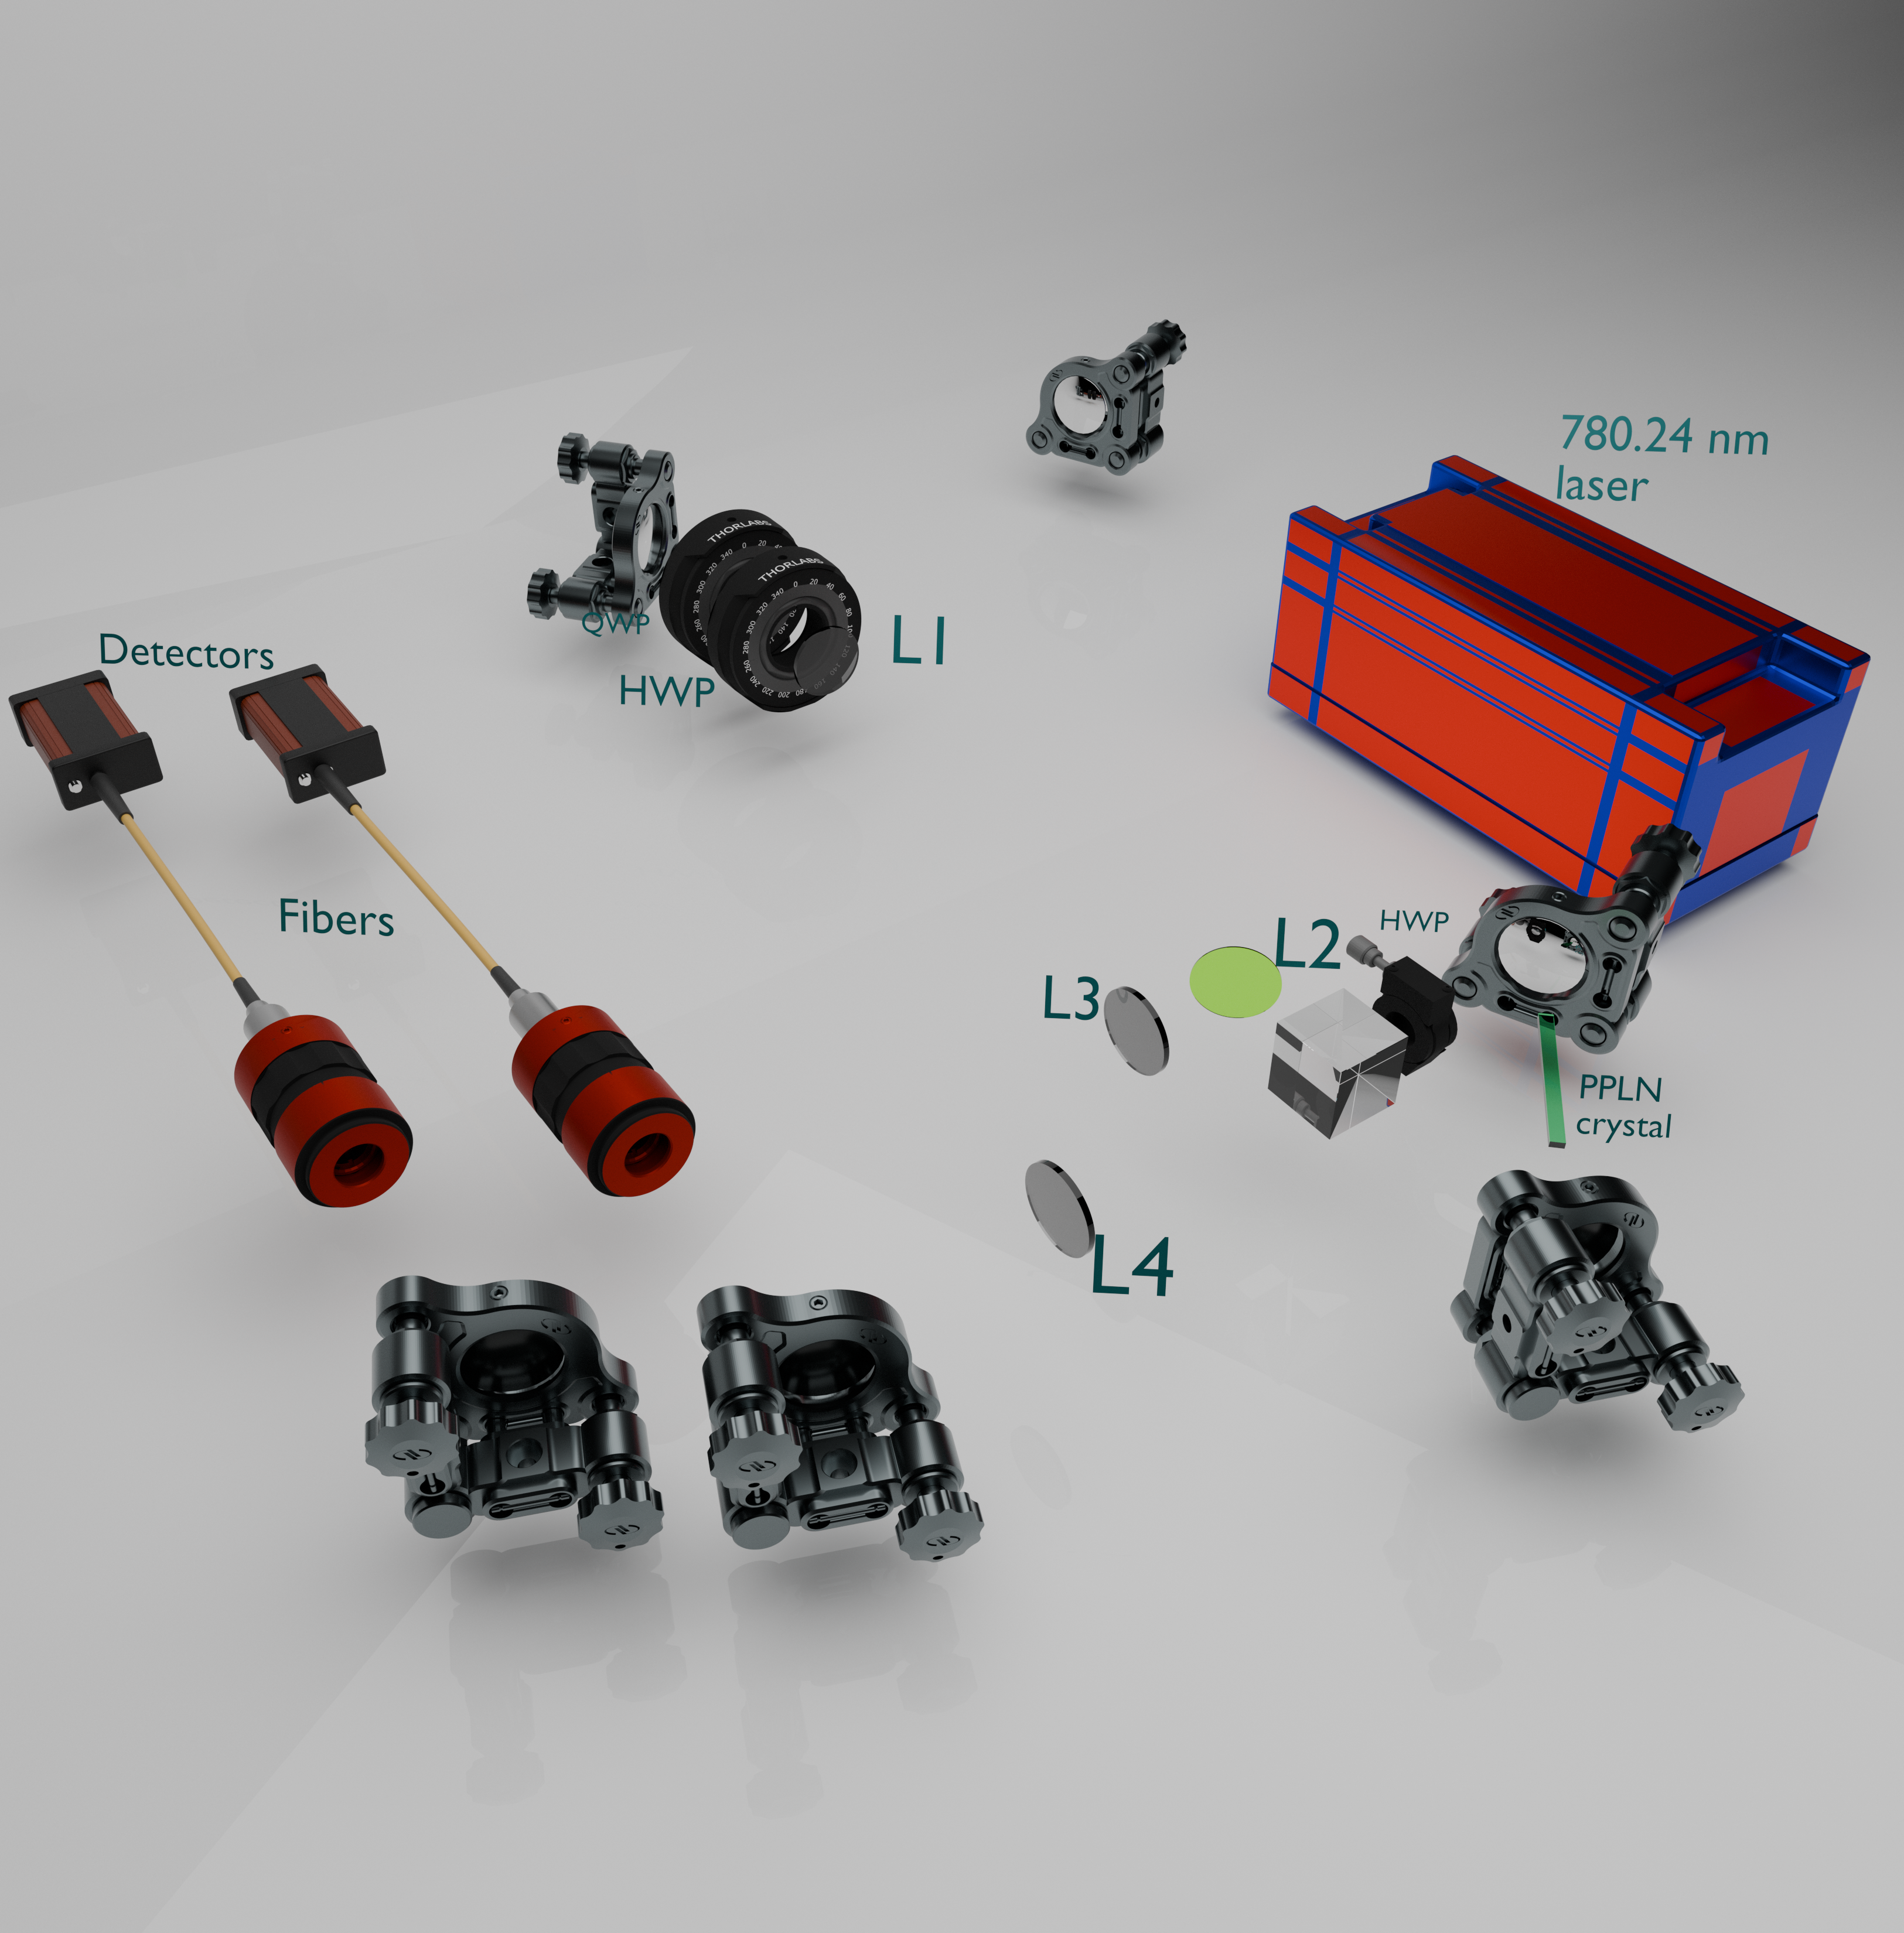
\includegraphics[width=0.95\textwidth]{~/Notes/PhDNotes/PhDTopicDefenseAbstract/Seminar/Presentation/Images/SagnacWithSomeAddedColoursV3.png}
	\end{center}
	\caption{}\label{fig:}
\end{figure}

\section{Contents and introduction}
Today I will be speaking to you about a part of my thesis, which is generating and teleporting entanglement for quantum networks. I will begin with a bit of theory,
where I will explain the basics of the Spontaneous Parametric Downconversion (SPDC). Here I will speak a bit about Phase Matching and how we try to optimize it in the lab. I will also
speak a bit about how we plan on Distributing Entanglement, so Quantum Teleportation and Entanglement Swapping.
Then I will speak about the present state that we are dealing with in the lab and how far we have gone so far.

\section{Motivation}
My project is in the scope of the SiQUID project. The goal of it is to demonstrate that a slovenian quantum network is possible to make,
train young researchers in the field of Quantum Technologies, as well as creating the sources of entanglement needed for entanglement based Quantum Key Distribution.
The main goal for me in this regard would be to create a bright source of polarization entanglemed photon pairs using a Sagnac interferometer.
The reason we chose a Sagnac in this case is due to its vibrational stability, and it's a convenient way to do so as it allows for a compact design.
A possible downside to this is that the alignment of this type of interferometer is a bit tedious, as you have to perfectly overlap two beams within the interferometer,
and in the crystal, and there is coupling between the various degrees of freedom that we have available to us.

\section{Theory}
\subsection{Spontaneous Parametric Downconversion}
Before talking about entanglement, we need to know how to generate photon pairs.
SPDC is a process in which a pump photon of frequency $\omega_p$ gets "downconverted" to two photons of lower frequency,
usually denoted as $\omega_s$ and $\omega_i$. These output photons can have the same frequency,
and thus this can be a degenerate process, or they can have different frequencies, being non-degenerate.
When we started this entire design process, we wanted to have a degenerate frequencies, as we would be able to separate
the two photons based on their polarization. This design utilited a type-II process, meaning that we would be able 
to separate the two photons on the output of the PBS.

\subsection{Phase Matching}
What is Phase Matching? Phase matching are the conditions at which some process will happen.
In the case of SPDC the Phase Matching conditions are energy conservation ($\hbar \omega_p = \hbar \omega_s + \hbar \omega_i$),
and momentum conservation ($k_p = k_s + k_i$). The efficiency of this process is also dictated by how well we satisfy these 
two conditions - being slightly off from $\Delta k = 0$ could result in large losses of efficiency.
% DONE NOTE: Add a slide after Phase Matching slide regarding type-0,-I,-II. DONE
% DONE NOTE: Mention the crystal properties - anisotropic stuff DONE
% NOTE: Add for quasi phase matching

\subsection{Crystals}
An important step is to choose the correct material for the job. In this case, no ordinary material can be used, 
as the phase matching condition $k_1 + k_2 = k_3 = \frac{n \omega_3}{c} = \frac{n \omega_1}{c} + \frac{n \omega_2}{c}$ is
impossible to satisfy in most cases as
$n_1 \left(	\omega_1 \right) < n_2 \left( \omega_2 \right) < n_3 \left(	\omega_3 \right)$ for $\omega_1 < \omega_2 < \omega_3$.

\subsection{Crystal Size}
Before periodic poling you could only have a limited size of the nonlinear material along the propagation direction.
This means that you would only be able to generate broad signals out of the crystals and at lower intensities, as the 
intensity and bandwidth of the process goes proportionally to $I \propto \text{sinc}^2\left(\frac{L \Delta k}{2}\right)$.
Today we have periodic poling available to us which allows us to create oppositely oriented fields inside the
crystal. This allows for higher photon generation rates, longer crystals and more narrow bandwidths.

\subsection{Types of processes}
There are three different types of phase matching.
\begin{itemize}
	\item Type-0 is one in which a photon of some linear polarization, say $\ket{H}$ gets downconverted
into two photons of lower energies of the same polarization - o $\rightarrow$ o + o. This process used to be physically impossible to produce 
as the phase matching condition $k_1 + k_2 = k_3 = \frac{n \omega_3}{c} = \frac{n \omega_1}{c} + \frac{n \omega_2}{c}$ is impossible to achieve
in most cases.
	\item Type-I is similar to type-0, except that the produced two photons are orthogonally polarized to the input photon - o $\rightarrow$ e + e
	\item In type-II instead you get two orthogonal polarizations out from the crystal. e $\rightarrow$ e + o
\end{itemize}

\subsection{Phase Matching Temperature}
The first important step is to determine the correct Phase Matching Temperature for our crystal. For different types of poling
periods these temperatures will vary, and in general, the lower the poling period the higher the Phase Matching Temperature.
The opposite seems to be true for the temperature bandwidth, which would be the acceptable temperature range for the material.
Similarly, one should not heat up certain crystals too much as this could destroy the Periodic Poling properties of the material.
For Periodically Poled Lithium Niobate (PPLN), the safe operating regime up to around 200 °C.

\subsection{Bandwidths}
Next would be the bandwidth of the process. In general, you would like it to be as narrow as possible - especially for certain
applications as entanglement swapping, and there are other methods to achieve this which I won't go into now. In general,
type-II processes are much more narrow than type-0 ones. In the plot I have on the slide, there's about a factor of 120 in 
bandwidth difference. This is why Type-II was the primary choice for our group. Unfortunately, this also comes at the price 
of reduced intensity. The difference in intensity was around 25 times lower compared to the type-0 crystal which led to us
using it in the end design.

\subsection{State of the Art}

\subsection{Different Designs}

\section{Entanglement}
If we have two systems, $\ket{\psi_i}$ and $\ket{\phi_i}$ described by two seperate Hilbert spaces, the state of those two systems can be described as 
a tensor product $\ket{\psi_i} \otimes \ket{\phi_i}$ of their state spaces. You can write this as a Schmidt decomposition: $\ket{\xi} = \sum_{i,j} 
a_{ij} \ket{\psi_i}\ket{phi_i} \rightarrow \sum_i b_i \ket{\psi_i'} \ket{\phi_i'}$. If $b_i \ne 0$ and $b_{i \ne j} = 0$ the state is said to be separable.
If more than one $b_i \ne 0$ then $\ket{\xi}$ is said to be entangled, and the states can no longer be described without their comprising states.
An example of entangled states are Bell states, they are also maximally entangled:

\begin{center}
	\begin{aligned}
		\begin{equation}
			\ket{\Psi^-} &= \frac{1}{\sqrt{2}} \left( \ket{0}\ket{1} - \ket{1}\ket{0} \right)\\
			\ket{\Psi^+} &= \frac{1}{\sqrt{2}} \left( \ket{0}\ket{1} + \ket{1}\ket{0} \right)\\
			\ket{\Phi^-} &= \frac{1}{\sqrt{2}} \left( \ket{0}\ket{0} - \ket{1}\ket{1} \right)\\
			\ket{\Phi^+} &= \frac{1}{\sqrt{2}} \left( \ket{0}\ket{0} + \ket{1}\ket{1} \right)
		\end{equation}
	\label{eq:bsm}
	\end{aligned}
\end{center}

\subsection{Why do we care about entanglement?}
Entanglement sources have many applications. Some notable ones are Quantum Computation, Quantum Imaging, and Quantum Sensing.
As we wish to distribute these entangled states over long distances, due to fiber losses it isn't viable to do so 
over distances larger than a couple hundred kilometers.
\begin{center}
	\begin{table}[h]
		\caption{Relevant fiber loss. \textit{Source: Thorlabs}}
		\label{tab:fiberloss}
		\begin{tabular}{|c|c|c|c|c|c|c|}
			\hline
			$\lambda$ [nm] & 430 & 532 & 780 & 1310 & 1550 & 1900\\
			\hline
			Loss [dB/km] & 50 & 30 & 12 & 0.32 &  0.18 & 5\\
			\hline
		\end{tabular}
	\end{table}
\end{center}
\begin{exampleblock}{Example: Loss in fiber for 1550/1560 nm}
	200 km of fiber \rightarrow -36 dB \rightarrow $10^4$ loss.
	Start with 1 W, end up with 0.0001 W.
\end{exampleblock}
Due to this, it would be desirable to have a more robust way to transport photons from A to B.
In our case, we generate a pair of $\ket{V}$ polarized photons in each of the branches of the Sagnac interferometer, totalling
to 4 photons being created "at the same time". This leads us to the entangled state for type-0 SPDC:
\begin{equation*}
	\ket{\Psi_{p}} = \frac{1}{\sqrt{2}} ( a_{H}^{\dagger} ( \omega_p ) + a_{V}^{\dagger} ( \omega_p ) )\ket{0}\\
\end{equation*}
\begin{minipage}[l]{0.48\textwidth}
	\begin{equation}
		\begin{aligned}
			\ket{\Psi_{\text{Type-2}}} &= \frac{1}{\sqrt{2}}(\sin(\alpha)a_{H}^{\dagger}(\omega_s)a_{V}^{\dagger}(\omega_i)+\\
								&\cos(\alpha)a_{V}^{\dagger}(\omega_i)a_{H}^{\dagger}(\omega_s))\ket{0}\\
		\end{aligned}
	\end{equation}
\end{minipage}
\begin{minipage}[r]{0.48\textwidth}
\begin{equation}
	\begin{aligned}
		\ket{\Psi_{\text{Type-0}}} &= \frac{1}{\sqrt{2}}(\sin(\alpha)a_{H}^{\dagger}(\omega_s)a_{H}^{\dagger}(\omega_i)+\\
								   &\cos(\alpha)a_{V}^{\dagger}(\omega_i)a_{V}^{\dagger}(\omega_s))\ket{0}
	\end{aligned}
\end{equation}
\end{minipage}

\par as one branch of the phons will be rotated in polarization due to a wave plate being in one of the branches of the Sagnac interferometer.
The reason why this is important is that if the conditions for this to happen are satisfied, you can no longer 
predict the result of the polarization measurement. You can no longer tell which photon is which and from where it came from.
But the measurements will be perfectly anti-correlated in polarization. 

\subsection{Distributing Entanglement}
Due to condisderable losses in fibers it is not feasible to transport entangled photons over distances greater than a few hundred kilometers. Thus 
we must find a different solution to long distance Entanglement Dirstribution. This could be solved with quantum repeater, but currently one does not exist, 
or is difficult to create. That being said, it is reasonable to establish an entanglement swapping network beforehand.

\subsubsection{Quantum Teleportation}
The basis of Quantum Teleportation is that the sender and receiver share an initial entangled pair - in our case polarization entangled photons of the sort described
above, then perform a Bell State Measurement (BSM) on the receiving entangled photon and an initial state which we would like to teleport to the receiver. 

\begin{description}
	\item[Bell State Measurement (BSM)] 
		A Bell State Measurement is a coincidence measurement between different detectors. The simplest one would
		be the $\ket{\Psi^-}$ of \ref{eq:bsm} measurement. In it you only have a 50:50 beam splitter and two detectors. The only
		time both photons will fall on their own separate detector is when either both of them get transmitted,
		or both get reflected. 
\end{description}

Then we report the result of the BSM via a classical communications channel to the receiver. This same procedure does not work if the entangled pair does 
not exist.
The amazing thing is that this should work regardless of the distance between the entangled states, and doesn't vialate any causality laws, as the cassical message
is being sent at most at the speed of causality to the receiver.


\subsubsection{Entanglement Swapping}
\section{Present State}
\subsection{Parameters}
\subsection{Building a Sagnac interferometer}

\end{document}
